% Teaching article for the American Journal of Physics, in AJP's manuscript format (REVTeX, Phys. Rev. B preprint
% style, superscript endnotes with article titles and page ranges).
% Build with:  latexmk -pdf main.tex      (from this folder)
% Figures:     Rscript paper/figures/make_figures.R      (from the repository root)
% To estimate the length in AJP's two-column journal format, replace "preprint" by "reprint".
\documentclass[aps,prb,preprint,amsmath,amssymb,nofootinbib,longbibliography]{revtex4-2}

% Shared by main.tex and supplementary.tex. AJP reviews anonymously: the first submission leaves out the author,
% affiliation and acknowledgments, and the citation of the code, which names the authors. Set \anonymousfalse for
% the version with them (after conditional acceptance).
\newif\ifanonymous
\anonymoustrue
\newcommand{\codecite}{\ifanonymous\cite{nnqs_code_anon}\else\cite{nnqs_code}\fi}
   % \anonymoustrue for review: no author, acknowledgments or named code citation

\usepackage{graphicx}
\usepackage{bm}
\usepackage{braket}
\usepackage{xcolor}
\usepackage{algpseudocode}
\usepackage[colorlinks=true,allcolors=blue!50!black]{hyperref}

\newcommand{\todo}[1]{\textcolor{red}{[TODO: #1]}}
\newcommand{\ev}[1]{\left\langle #1 \right\rangle}
\newcommand{\Eloc}{E_{\mathrm{loc}}}
\newcommand{\dtau}{\delta\tau}
\renewcommand{\Re}{\operatorname{Re}}
\renewcommand{\Im}{\operatorname{Im}}

\begin{document}

\title{Neural-network quantum states as imaginary-time evolution:\\ a worked example on the transverse-field Ising chain}

\ifanonymous\else
\author{Austin Chase Bullock}
\email{austin@acbbullock.com}
\affiliation{Independent researcher}
\fi

\date{\today}

\begin{abstract}
A restricted Boltzmann machine with complex parameters can represent the ground state of a quantum spin chain, and
stochastic reconfiguration trains it by variational Monte Carlo. We derive stochastic reconfiguration from
imaginary-time evolution with McLachlan's variational principle. The derivation shows that each training step is a
least-squares fit of the fluctuations of the local energy by the fluctuations of the logarithmic derivatives of the
wave function. We give a short implementation in standard Fortran 2018 that runs in parallel on coarray images. The
transverse-field Ising chain maps onto free fermions, so every result is checked against the exact solution. Deep in
the ordered phase, chains of 1000 and 1024 spins reach the exact ground-state energy to within 3 parts in $10^5$,
and their spin correlations agree with the exact ones to better than $10^{-3}$ on average. Near and beyond the
quantum critical point, the same method with 16 hidden units on 64 spins stays too ordered, and its energy is 2--5\%
too high. We also show how five small implementation errors, each easy to make, spoil the results, and how a
variational energy below the exact ground-state energy exposes a broken sampler. The code and data are openly
available.
\end{abstract}

\maketitle

%======================================================================================================================
\section{Introduction}
\label{sec:intro}

The state of $n$ spins-$\frac12$ is a vector in a space of dimension $2^n$, so every practical method for large
systems needs a compressed description of it. In the variational method, a trial state $\ket{\psi_\alpha}$ with
parameters $\alpha$ is adjusted to lower the energy $E(\alpha) = \bra{\psi_\alpha}H\ket{\psi_\alpha} /
\braket{\psi_\alpha|\psi_\alpha}$, which can never fall below the exact ground-state energy $E_0$. Variational Monte
Carlo (VMC) estimates $E(\alpha)$ and its derivatives from configurations sampled according to
$|\psi_\alpha|^2$.\cite{becca2017}

Carleo and Troyer\cite{carleo2017} used a restricted Boltzmann machine (RBM), a simple neural network, as the trial
state and trained it with stochastic reconfiguration (SR).\cite{sorella1998,sorella2001} Such \emph{neural-network
quantum states} are now a field of their own,\cite{lange2024} with mature software.\cite{netket2022} For a student,
however, SR usually appears as a recipe: precondition the energy gradient with the covariance matrix of the
logarithmic derivatives. Where that matrix comes from, and why the recipe finds the ground state, is left to the
specialist literature, and large packages are hard to read line by line.

This article fills that gap with a complete worked example. Section~\ref{sec:sr} derives SR from imaginary-time
evolution with McLachlan's variational principle.\cite{mclachlan1964} None of the ingredients is new. Sorella
introduced SR as the projection of imaginary-time (power-method) evolution onto the variational
subspace,\cite{sorella1998,sorella2001,becca2017} the same McLachlan projection underlies variational imaginary-time
evolution on quantum computers,\cite{mcardle2019,yuan2019} and the least-squares form is the starting point of recent
solvers for large networks.\cite{chen2024,rende2024} What we add is a self-contained, one-page account at the level
of a first graduate course in quantum mechanics, which shows that SR is an ordinary least-squares problem. We apply
it to the transverse-field Ising chain (Sec.~\ref{sec:model}), whose exact solution lets us judge every result, with
a Fortran module of about 700 lines (Sec.~\ref{sec:implementation}).\codecite\ The results
(Sec.~\ref{sec:results}) include a regime where the method works very well and one where it does not.
Section~\ref{sec:pitfalls} documents five implementation errors that we made and their measurable effects, and
Sec.~\ref{sec:discussion} closes with suggested problems.

%======================================================================================================================
\section{The transverse-field Ising chain}
\label{sec:model}

We study an open chain of $n$ spins-$\frac12$ with Hamiltonian
\begin{equation}
  H = -J \sum_{j=1}^{n-1} \sigma^z_j \sigma^z_{j+1} - B \sum_{j=1}^{n} \sigma^x_j ,
  \label{eq:hamiltonian}
\end{equation}
where $\sigma^{x,z}_j$ are Pauli matrices acting on spin $j$. The coupling favors aligned neighbors for $J > 0$
(ferromagnet) and anti-aligned ones for $J < 0$ (antiferromagnet), while the transverse field $B$ tries to point every
spin along $x$. Their competition gives a quantum phase transition at $|B| = |J|$. For $|B| < |J|$ the chain is
ordered: in the thermodynamic limit $\ev{\sigma^z_i\sigma^z_k}$ tends to $m^2 = [1 - (B/J)^2]^{1/4}$ as $|i - k| \to
\infty$.\cite{pfeuty1970} For $|B| > |J|$ the correlations decay exponentially.

\paragraph*{Signs do not matter.}
The unitary $U = \prod_{j\,\mathrm{even}} \sigma^x_j$ flips $\sigma^z$ on every second site, so $U H(J,B) U^\dagger
= H(-J,B)$; likewise $V = \prod_j \sigma^z_j$ maps $B \to -B$. All four sign choices therefore have the same
spectrum, and the antiferromagnet's correlations are those of the ferromagnet with a staggered sign:
\begin{equation}
  \ev{\sigma^z_i \sigma^z_k}_{-J} = (-1)^{k-i} \ev{\sigma^z_i \sigma^z_k}_{J} .
  \label{eq:stagger}
\end{equation}
Our program trains on $H(|J|,|B|)$ and staggers the measured correlations when $J < 0$. This is more than a
convenience. With $J = -0.5$, $B = 0.1$, $m = 16$ hidden units, $N_s = 256$ samples on one image, $\dtau = 0.01$ and
1000 epochs, training on $H(J,B)$ itself ends 20\% above $E_0$ for 64 spins (median of 5 seeds, range 17--22\%) and
19\% above for 256 spins (3 seeds). With the sign change the error is 0.005\% for 64 spins and within the Monte Carlo
noise for 256. Only for 12 spins do both work. A likely reason is that the initial weights favor a uniformly
magnetized state, which is close to the ferromagnetic ground state and far from the antiferromagnetic one.

\paragraph*{Exact solution.}
The Jordan--Wigner transformation maps Eq.~\eqref{eq:hamiltonian} onto a chain of free
fermions.\cite{lieb1961,pfeuty1970,mbeng2024} The ground-state energy of the open chain is (supplementary material,
Sec.~S2)
\begin{equation}
  E_0 = -\sum_{k=1}^{n} \lambda_k ,
  \label{eq:exact-energy}
\end{equation}
where $\lambda_k$ are the singular values of the $n\times n$ upper-bidiagonal matrix $M$ with $M_{jj} = |B|$ and
$M_{j,j+1} = |J|$. One singular-value decomposition gives $E_0$ for thousands of spins, and it agrees with exact
diagonalization of 6--8 spins, including the critical point, to machine precision. Spin correlations are
determinants of fermionic two-point functions (Sec.~S2).

%======================================================================================================================
\section{A neural-network wave function}
\label{sec:rbm}

We label basis states by $s = (s_1,\ldots,s_n)$ with $s_j \in \{0,1\}$, where $s_j = 0$ means spin up, so that
$\sigma^z_j\ket{s} = \sigma_j\ket{s}$ with $\sigma_j = 1 - 2s_j$, and write $\ket{\psi_\alpha} = \sum_s
\psi_\alpha(s)\ket{s}$. An RBM has $n$ visible units $s_j$ and $m$ hidden units $h_i \in \{0,1\}$, with no
connections within a layer. Following Ref.~\onlinecite{carleo2017}, we give it complex parameters and sum out the
hidden layer:
\begin{align}
  \psi_\alpha(s) &= \sum_{h \in \{0,1\}^m} \exp\!\Big(\sum_j a_j s_j + \sum_i c_i h_i + \sum_{ij} h_i W_{ij} s_j \Big)
  \nonumber \\
  &= e^{\sum_j a_j s_j} \prod_{i=1}^{m} \big(1 + e^{\theta_i(s)}\big),
  \label{eq:rbm}
\end{align}
with $\theta_i(s) = c_i + \sum_{j} W_{ij} s_j$. The sum factorizes because each $h_i$ appears in only one exponent, so
an amplitude costs $\mathcal{O}(nm)$ operations. We keep the $n$ visible biases $a$ real (Sec.~\ref{sec:real}) and let
the $m$ hidden biases $c$ and the $nm$ weights $W$ be complex, so that $\psi_\alpha$ can carry signs and phases. With
enough hidden units an RBM can represent any distribution over $s$;\cite{leroux2008} in practice the ratio $m/n$
controls the accuracy.

Everything below needs only the \emph{logarithmic derivatives} $O_k(s) = \partial \ln\psi_\alpha(s)/\partial
\alpha_k$, which are
\begin{equation}
  O_{a_j} = s_j, \quad O_{c_i} = \varsigma(\theta_i), \quad O_{W_{ij}} = s_j\,\varsigma(\theta_i),
  \label{eq:logderiv}
\end{equation}
with the logistic function $\varsigma(z) = e^z/(1+e^z)$. Since $\psi_\alpha$ depends on $c$ and $W$ but not on their
complex conjugates, it is holomorphic in them, and these are ordinary complex derivatives.

%======================================================================================================================
\section{Variational Monte Carlo}
\label{sec:vmc}

Let $p_\alpha(s) = |\psi_\alpha(s)|^2 / \sum_{s'} |\psi_\alpha(s')|^2$ be the Born probability of configuration $s$,
and write $\ev{f} = \sum_s p_\alpha(s) f(s)$ for averages over it. Inserting a complete set of states shows that the
variational energy is the average of the \emph{local energy}:
\begin{equation}
  E(\alpha) = \frac{\bra{\psi_\alpha}H\ket{\psi_\alpha}}{\braket{\psi_\alpha|\psi_\alpha}} = \ev{\Eloc},
  \label{eq:energy}
\end{equation}
with
\begin{equation}
  \Eloc(s) = \sum_{s'} \bra{s}H\ket{s'} \frac{\psi_\alpha(s')}{\psi_\alpha(s)} .
  \label{eq:eloc-def}
\end{equation}
For the Ising chain, each configuration $s$ connects to itself through the $\sigma^z\sigma^z$ terms and to the $n$
configurations $s^{(j)}$ with spin $j$ flipped through the $\sigma^x$ terms:
\begin{equation}
  \Eloc(s) = -J \sum_{j=1}^{n-1} \sigma_j\sigma_{j+1} - B \sum_{j=1}^{n} \frac{\psi_\alpha(s^{(j)})}{\psi_\alpha(s)} ,
  \label{eq:eloc}
\end{equation}
with
\begin{equation}
  \ln\frac{\psi_\alpha(s^{(j)})}{\psi_\alpha(s)} = a_j\sigma_j + \sum_{i=1}^m \Big[\ln\big(1+e^{\theta_i + W_{ij}
  \sigma_j}\big) - \ln\big(1+e^{\theta_i}\big)\Big],
  \label{eq:ratio}
\end{equation}
since flipping spin $j$ changes $s_j$ by $\sigma_j$. Only ratios of amplitudes appear, so the normalization of
$\psi_\alpha$ is never needed. If the $\theta_i(s)$ are kept in memory, each ratio costs $\mathcal{O}(m)$ operations
and each local energy costs $\mathcal{O}(nm)$. Although $E(\alpha)$ is real, $\Eloc(s)$ is complex whenever
$\psi_\alpha$ is; only its average is real. This point matters for the gradient (Sec.~\ref{sec:pitfalls}).

\paragraph*{Sampling.}
We draw configurations from $p_\alpha$ with the Metropolis--Hastings algorithm.\cite{metropolis1953}
Each step proposes flipping one spin chosen at random and accepts the flip with probability $\min\{1,
|\psi_\alpha(s^{(j)})/\psi_\alpha(s)|^2\}$, using Eq.~\eqref{eq:ratio}. Averages over $N_s$ samples estimate
$\ev{\cdot}$. The statistical error of the energy estimate is approximately $\sqrt{\mathrm{var}(\Eloc)/N_s}$, but only
if the samples are independent; correlated samples make this estimate too small.\cite{flyvbjerg1989}

\paragraph*{Zero variance.}
If $\psi_\alpha$ is an exact eigenstate of $H$, then $\Eloc(s)$ equals the eigenvalue for every $s$ and its variance
vanishes. The variance of the local energy is therefore a measure of quality that, unlike the error in the energy,
does not require knowing $E_0$.

%======================================================================================================================
\section{Stochastic reconfiguration from imaginary-time evolution}
\label{sec:sr}

\subsection{Imaginary-time evolution}

Expand any state in the eigenstates of $H$, $\ket{\Phi} = \sum_k b_k \ket{k}$ with energies $E_0 < E_1 \le \cdots$.
Then
\begin{equation}
  e^{-\tau H}\ket{\Phi} = e^{-\tau E_0}\Big[b_0\ket{0} + \sum_{k>0} e^{-\tau (E_k - E_0)} b_k\ket{k}\Big],
\end{equation}
so for large $\tau$ only the ground state survives, provided $b_0 = \braket{0|\Phi} \neq 0$. The parameter $\tau$
plays the role of an imaginary time, because $e^{-\tau H}$ is the time-evolution operator $e^{-itH}$ with $t = -i\tau$.
Dropping the overall factor, which changes only the norm, the state obeys
\begin{equation}
  \frac{d}{d\tau}\ket{\Phi} = -(H - E)\ket{\Phi}, \quad E = \frac{\bra{\Phi}H\ket{\Phi}}{\braket{\Phi|\Phi}} .
  \label{eq:imaginary-time}
\end{equation}
Subtracting $E$ keeps the norm constant to first order but does not change the physical state, which is the ray
spanned by $\ket{\Phi}$.

\subsection{Projecting onto the variational manifold}

We cannot evolve the full $2^n$-component vector, but we can let the parameters depend on $\tau$. Then
$\frac{d}{d\tau}\ket{\psi_\alpha} = \sum_k \dot\alpha_k\,\partial_k\ket{\psi_\alpha}$, where $\dot\alpha_k =
d\alpha_k/d\tau$, is confined to the tangent space of the manifold of RBM states, whereas the right-hand side of
Eq.~\eqref{eq:imaginary-time} is not. McLachlan's principle\cite{mclachlan1964} picks the velocity $\dot\alpha$ that
makes the two sides as close as possible in norm. Since multiplying the state by a complex number changes neither
the physical state nor the energy, we also allow a free term $\eta\ket{\psi_\alpha}$ with $\eta \in \mathbb{C}$, and
minimize
\begin{equation}
  D(\dot\alpha,\eta) = \frac{\big\| \big(\sum_k \dot\alpha_k \partial_k + \eta + H - E\big)\ket{\psi_\alpha} \big\|^2}
  {\braket{\psi_\alpha|\psi_\alpha}} .
\end{equation}
Since $\partial_k\psi_\alpha(s) = O_k(s)\psi_\alpha(s)$ and $(H\psi_\alpha)(s) = \Eloc(s)\psi_\alpha(s)$, each term
is a function of $s$ times $\psi_\alpha(s)$, and
\begin{equation}
  D = \Big\langle \Big| \sum_k \dot\alpha_k O_k + \eta + \Eloc - E \Big|^2 \Big\rangle .
\end{equation}
Minimizing over $\eta$ simply removes the mean of everything inside the bars, $\eta = -\sum_k \dot\alpha_k
\ev{O_k}$. With the fluctuations $\Delta O_k = O_k - \ev{O_k}$ and $\Delta\Eloc = \Eloc - E$, this leaves
\begin{equation}
  \boxed{\; D(\dot\alpha) = \Big\langle \Big| \sum_k \dot\alpha_k\, \Delta O_k + \Delta\Eloc \Big|^2 \Big\rangle \;}
  \label{eq:least-squares}
\end{equation}
This is the key equation of the article, and the starting point of the minimum-step SR of
Ref.~\onlinecite{chen2024}. The best imaginary-time step is a weighted least-squares fit: we choose a combination of
the log-derivative fluctuations $\Delta O_k(s)$ that cancels the local-energy fluctuations $\Delta\Eloc(s)$ as well as
possible, with each configuration weighted by its Born probability.

Setting $\partial D/\partial\dot\alpha_k^* = 0$ gives the normal equations of this fit,
\begin{equation}
  \sum_l S_{kl}\,\dot\alpha_l = -F_k ,
  \label{eq:sr}
\end{equation}
with the matrix and vector
\begin{align}
  S_{kl} &= \ev{\Delta O_k^* \Delta O_l} = \ev{O_k^* O_l} - \ev{O_k^*}\ev{O_l}, \label{eq:S} \\
  F_k &= \ev{\Delta O_k^* \Delta\Eloc} = \ev{O_k^* \Eloc} - \ev{O_k^*}\ev{\Eloc} . \label{eq:F}
\end{align}
These are the equations of stochastic reconfiguration.\cite{sorella1998,carleo2017} Integrating them
with forward Euler steps of size $\dtau$ gives the update
\begin{equation}
  \alpha \leftarrow \alpha - \dtau\, S^{-1} F .
  \label{eq:update}
\end{equation}
For a parametrization like ours, which is holomorphic in its complex parameters, the other common variational
principles (Dirac--Frenkel and the time-dependent variational principle) lead to the same
equations.\cite{yuan2019}

\subsection{What the two matrices mean}

The vector $F$ is the gradient of the energy. Differentiating $E(\alpha)$ with respect to $\alpha_k^*$, which acts only
on the bra, gives $\partial E/\partial\alpha_k^* = F_k$. Hence $dE = 2\Re\sum_k F_k^*\,d\alpha_k$, and along the SR
flow
\begin{equation}
  \frac{dE}{d\tau} = -2\,F^\dagger S^{-1} F \le 0 .
  \label{eq:descent}
\end{equation}
The energy decreases monotonically, and it stops changing only where $F = 0$, that is, at a stationary point of
$E(\alpha)$ on the manifold.

The matrix $S$ is the metric of the manifold: $\sum_{kl}\delta\alpha_k^* S_{kl}\delta\alpha_l$ is the squared
distance between the normalized states $\psi_\alpha$ and $\psi_{\alpha+\delta\alpha}$, with changes of norm and global
phase removed (the Fubini--Study metric). Plain gradient descent, $\dot\alpha = -F$, measures step sizes in parameter
space, where they mean little. SR measures them by how much the physical state changes, which makes it the
quantum analogue of the natural gradient of machine learning.\cite{amari1998,stokes2020}

The minimum of Eq.~\eqref{eq:least-squares},
\begin{equation}
  D_{\min} = \mathrm{var}(\Eloc) - F^\dagger S^{-1}F \ge 0,
  \label{eq:residual}
\end{equation}
measures how much of the exact imaginary-time evolution the manifold fails to capture. Its real-time
counterpart is used to monitor the accuracy of neural-network simulations of dynamics.\cite{schmitt2020} When the RBM can follow the
exact flow, $D_{\min} = 0$ and, by the argument of the previous subsection, training converges to the ground state.

\subsection{Real parameters}
\label{sec:real}

If a parameter is restricted to be real, the minimization is over real $\dot\alpha_k$ only. For a block of real
parameters this replaces Eq.~\eqref{eq:sr} by $(\Re S)\,\dot\alpha = -\Re F$ (Problem~\ref{prob:real}). We keep the
visible biases $a$ real. Their log derivatives $O_{a_j} = s_j$ are real, so the real parts of $a$ already describe
everything that the visible biases can do to the magnitudes $|\psi_\alpha(s)|$. Phases are left to $c$ and $W$.

\subsection{From equations to an algorithm}
\label{sec:approximations}

Three practical issues remain.

\emph{Estimation.} All averages are replaced by averages over the $N_s$ sampled configurations. The fit of
Eq.~\eqref{eq:least-squares} then becomes an explicit least-squares problem over the samples. With
$X_{ik} = \Delta O_k(s_i)/\sqrt{N_s}$ and $e_i = \Delta\Eloc(s_i)/\sqrt{N_s}$, we have $S = X^\dagger X$ and
$F = X^\dagger e$.

\emph{Regularization.} A sample estimate of $S$ has rank at most $N_s - 1$, so it is singular whenever there are more
parameters than samples. $S$ is also nearly singular when parameters are redundant. We add a small diagonal shift,
$S \to S + \epsilon\,\mathbb{1}$, which amounts to adding $\epsilon\|\dot\alpha\|^2$ to $D$ and penalizes large
steps.

\emph{Cost.} The full $S$ has $N_p^2$ entries, where $N_p = n + m + nm$ is the number of parameters. For $n = 1024$
and $m = 64$, $N_p = 66\,624$, so $S$ would take tens of gigabytes and a dense solve would cost
$\mathcal{O}(N_p^3)$ operations. We therefore use a block-diagonal approximation. We keep one block for $a$, one for
$c$, and one $m\times m$ block for each column $W_{\cdot j}$ of the weights, and drop the correlations between
blocks. Each block's step is then the exact McLachlan step for that block alone. Because a block-diagonal part of a
positive-definite matrix is itself positive definite, Eq.~\eqref{eq:descent} still guarantees descent, but the step
is no longer the projected imaginary-time evolution. The exact step is also affordable: when $N_s < N_p$, the
identity $(X^\dagger X + \epsilon)^{-1}X^\dagger = X^\dagger(XX^\dagger + \epsilon)^{-1}$ reduces it to an
$N_s\times N_s$ solve.\cite{chen2024,rende2024} With the real biases $a$, we write every complex parameter as two
real ones, its real and imaginary parts, whose log derivatives are $O_k$ and $iO_k$. Stacking the real and imaginary
parts of the $N_s$ samples then gives a real $2N_s\times N_p'$ matrix $X$, with $N_p' = n + 2(m + nm)$ real
parameters, and the exact step needs only a real $2N_s\times 2N_s$ solve. We compare the two in
Sec.~\ref{sec:critical}.

%======================================================================================================================
\section{Implementation}
\label{sec:implementation}

The program\codecite\ is written in standard Fortran 2018. Its one module defines a derived type for the RBM,
with type-bound procedures for sampling, the local energy and the SR step. The supplementary material lists one
training run as pseudocode (Fig.~S1), every setting (Table~S1), and how the program samples and solves for each
block (Sec.~S1). All runs use $N_s = 256$ samples per image, a time
step $\dtau = 0.01$, a diagonal shift $\epsilon = 10^{-3}$ and 1000 epochs, in single precision, with $P = 4$ images unless stated
otherwise. The biases start at zero, and the weights at nearly uniform values close
to $W_{ij} = 0.01 - 0.005i$.

\paragraph*{Numerical stability.}
$\ln(1 + e^z)$ and $\varsigma(z)$ overflow for large $\Re z$. We evaluate them as $z + \ln(1 + e^{-z})$ and
$1/(1 + e^{-z})$ when $\Re z > 0$. These forms can differ from the naive ones by multiples of $2\pi i$, which leave
$\psi_\alpha$ unchanged. With this, single precision suffices: runs in double precision gave the same accuracy
(Sec.~\ref{sec:pitfalls}).

\paragraph*{Parallel images.}
Fortran 2008 coarrays and the collective subroutines of Fortran 2018\cite{reid2018} run $P$
copies (\emph{images}) of the program at once. At the start of each epoch the parameters are averaged over the
images with \texttt{co\_sum}, so every image samples the same $\psi_\alpha$. Each image then takes an SR step from its
own $N_s$ samples, and the next average combines the steps. The update is therefore $\alpha \to \alpha -
(\dtau/P)\sum_p S_p^{-1}F_p$, which is not exactly the step computed from all $PN_s$ samples together, since the mean
of $S_p^{-1}F_p$ is not $(\text{mean } S_p)^{-1}(\text{mean } F_p)$. The reported energy is the mean over images, and
its error is $\sqrt{\sum_p \sigma_p^2}/P$. Without coarrays the same source builds as a single-image program.

%======================================================================================================================
\section{Results}
\label{sec:results}

\subsection{Long chains in the ordered phase}

\begin{figure}[t]
  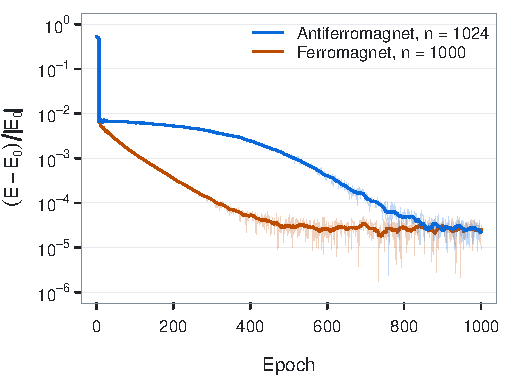
\includegraphics[width=\columnwidth]{figures/training.pdf}
  \caption{Relative error of the variational energy during training at $B = 0.1$, $|J| = 0.5$, with $m = 64$ hidden
  units and the settings of Sec.~\ref{sec:implementation}. Faint lines show each epoch, and solid lines a running mean
  over 21 epochs.}
  \label{fig:training}
\end{figure}

Figure~\ref{fig:training} shows two runs deep in the ordered phase, $B/|J| = 0.2$: an antiferromagnet of $n = 1024$
spins ($J = -0.5$) and a ferromagnet of $n = 1000$ spins ($J = 0.5$), both with $m = 64$ hidden units. Thanks to
Eq.~\eqref{eq:stagger}, the network learns the ferromagnetic ground state in both cases. Both runs fall below 1\%
error within 8 epochs, once the chain has ordered. The run with 1000 spins then converges steadily. The run with
1024 spins stays near 0.7\% for about 200 epochs before it converges. The correlations show that this plateau is not
caused by domain walls: from epoch 10 onward, no spin's correlation with the middle spin falls below 0.93, so the
chain is ordered from end to end. The
excess energy is in the short-range quantum fluctuations.

\begin{table}[b]
\caption{Final energies at $B = 0.1$, $|J| = 0.5$, $m = 64$, averaged over the last 128 epochs. The number in
parentheses is the statistical error in the last digit, from a blocking analysis.}
\label{tab:long}
\begin{ruledtabular}
\begin{tabular}{lccc}
Chain & $E$ & $E_0$ & $(E - E_0)/|E_0|$ \\
\hline
$n = 1024$, AFM & $-516.6286(6)$ & $-516.6430$ & $2.8\times 10^{-5}$ \\
$n = 1000$, FM & $-504.5097(6)$ & $-504.5227$ & $2.6\times 10^{-5}$ \\
\end{tabular}
\end{ruledtabular}
\end{table}

Table~\ref{tab:long} gives the final energies. We average the energy over the last 128 epochs and estimate its error
by blocking:\cite{flyvbjerg1989} we repeatedly average neighboring pairs of epochs and watch the standard error of
the mean. Here the error stays flat as the blocks grow, which shows that successive epoch energies are uncorrelated.
The remaining gap to $E_0$ is more than 20 times the error bar. It is the true variational error of the network, three
parts in $10^5$. The variance of the local energy gives the same picture without reference to $E_0$:
$\mathrm{var}(\Eloc)/E_0^2 \approx 9\times10^{-8}$ for both chains.

Error bars deserve care. The per-epoch error printed by the program, $\sqrt{\mathrm{var}(\Eloc)/(PN_s)}$, treats the
samples as independent. In the last 128 epochs it is about 0.0049, whereas the energies of successive epochs scatter
with a standard deviation of 0.0064. Samples one sweep apart are thus correlated enough that the true scatter is
about 30\% larger than the naive error.

The spin correlations $\ev{\sigma^z_c\sigma^z_j}$ with the middle spin $c$, averaged over the same 128 epochs, agree
with the exact correlations (supplementary material, Sec.~S2) to $3\times10^{-4}$ (ferromagnet) and $6\times10^{-4}$
(antiferromagnet), averaged over sites. At large distances both approach $m^2 = 0.98985$. The network breaks the
$\mathbb{Z}_2$ symmetry of the chain and settles into one of the two ordered states, with about 99.75\% of spins down
in the final samples. For $n \approx 1000$ the symmetric and broken states differ in energy by an exponentially small
amount. Moreover, $\sigma^z_c\sigma^z_j$ is invariant under the symmetry, so its average is the same in both states.

Each run took about 55 minutes on four images of an Intel Xeon w5-3435X, sharing the machine with other jobs.

\subsection{Across the quantum critical point}
\label{sec:critical}

\begin{figure}[t]
  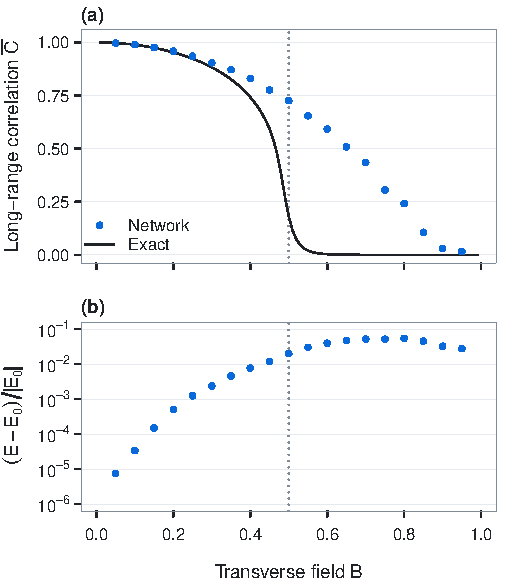
\includegraphics[width=\columnwidth]{figures/field_sweep.pdf}
  \caption{A ferromagnetic chain of $n = 64$ spins with $J = 0.5$ and $m = 16$, trained separately at each $B$.
  (a) Long-range correlation $\bar C$, the mean of $\ev{\sigma^z_c\sigma^z_j}$ over sites at least $n/4$ from the
  middle spin $c$, averaged over the last 100 epochs, compared with the exact value. (b) Relative error of the energy,
  averaged over the last 128 epochs. The dotted line marks the critical point $B = J$.}
  \label{fig:sweep}
\end{figure}

Figure~\ref{fig:sweep} shows what happens as the field increases. We use a smaller chain,
$n = 64$ with $m = 16$, trained independently at each of 19 fields. The error grows by four orders of magnitude, from
$10^{-5}$ at $B = 0.05$ to 2\% at the critical point. It peaks at about 5\% for $B = 0.65$--$0.8$ in the disordered
phase, and falls again as $B$ grows and the ground state approaches the simple product state with every spin along
$x$. Panel (a) shows how the network fails. It remains too ordered: at $B = 0.65$ its long-range correlation is still
0.5, whereas the exact correlation is essentially zero.

We have not found the cause, and we report the failure as it stands. Training five times longer does not cure it:
at $B = 0.8$ on one image, 5000 epochs lowered the error only from about 7\% to about 6\%.

\begin{table}[b]
\caption{Full $S$ against the block-diagonal $S$. Median relative error of the final Monte Carlo energy, in percent,
with the range over seeds in brackets. All runs used $J = 0.5$, $m = 16$, $N_s = 256$ on one image, $\dtau = 0.01$,
$\epsilon = 10^{-3}$, 1000 epochs, gfortran and single precision, with 5 seeds for $n = 64$ and 3 for $n = 256$. The
runs at $B = 0.25$, 0.4 and 0.65 are with the raw results (see Data availability).
With one image, the block-diagonal errors are larger than those of Fig.~\ref{fig:sweep}, which used four.}
\label{tab:fullsr}
\begin{ruledtabular}
\begin{tabular}{rlcc}
$n$ & $B$ & Block-diagonal $S$ & Full $S$ \\
\hline
64 & 0.10 & 0.005 [0.004, 0.009] & 0.007 [0.004, 0.027] \\
   & 0.50 & 2.3 [2.2, 2.5] & 1.7 [1.7, 2.0] \\
   & 0.80 & 7.1 [6.6, 7.2] & 3.6 [3.4, 3.9] \\
   & 0.95 & 6.5 [6.1, 13] & 2.7 [2.0, 3.0] \\
256 & 0.10 & $-0.002$ [$-0.002$, 0.004] & 7.0 [5.5, 9.8] \\
   & 0.50 & 1.8 [1.8, 2.0] & 4.7 [3.6, 7.1] \\
   & 0.80 & 7.2 [7.0, 7.3] & 8.5 [8.3, 8.6] \\
\end{tabular}
\end{ruledtabular}
\end{table}

A natural suspect is the block-diagonal approximation, which drops the correlations between the weights attached to
different spins just where the correlation length grows. Table~\ref{tab:fullsr} tests it by replacing the
block-diagonal $S$ with the full $S$, with everything else unchanged. For $n = 64$, the full $S$ makes no difference
in the ordered phase. It helps more the larger the field, and roughly halves the error at $B = 0.8$ and $0.95$. Even
so, the error stays at several percent. For $n = 256$ with the same 256 samples, the full $S$ is \emph{worse} at
every field, even deep in the ordered phase: at $B = 0.1$ it ends 7\% above $E_0$, where the block-diagonal $S$
reaches $E_0$ within the noise. We do not know why. One plausible reason is
that the full $S$ of the larger network, with 8480 real parameters, is estimated from only 256 samples, so it has
rank at most 510 and is dominated by sampling noise, whereas each block of the block-diagonal $S$ is small. The
approximation of $S$ is therefore part of the problem for the smaller chain, but not all of it, and the number of
samples matters as well.

%======================================================================================================================
\section{Five ways to get it subtly wrong}
\label{sec:pitfalls}

The first version of our program (2022--2024) gave plausible energies, 0.8\% above $E_0$ for the long chain, but
it contained errors that we later found. To measure each, we added to the released program a switch that puts it
back and ran a leave-one-out ablation (Table~\ref{tab:ablation}). The first version also put an Adam-type adaptive
step on top of SR and gave the weights a random ``kick'' whenever the error bar became small; both kept long chains
from converging and are absent from every row.

\begin{table*}[t]
\caption{Leave-one-out ablation. Each entry is the median relative error of the Monte Carlo energy, in percent, over
10 seeds ($n = 12$) or 5 seeds ($n = 256$). For $n = 12$, the number in brackets is the exact energy of the trained
state, summed over all $2^{12}$ configurations. All runs used $J = -0.5$, $N_s = 256$, $\dtau = 0.01$, 1000 epochs, a
single image, gfortran and single precision. ``All fixes'' is the program of Sec.~\ref{sec:implementation}; each
other row puts back the error named. Negative entries for $n = 256$ lie within the Monte Carlo noise of the final
epoch.}
\label{tab:ablation}
\begin{ruledtabular}
\begin{tabular}{lccc}
 & $n = 12$, $m = 12$ & $n = 12$, $m = 12$ & $n = 256$, $m = 16$ \\
Variant & $B = 0.1$ & $B = 0.5$ & $B = 0.1$ \\
\hline
All fixes & 0.005 [0.010] & 0.89 [0.89] & $-0.002$ \\
Chain restarted each epoch & $\mathbf{-0.027}$ [0.007] & 3.2 [2.7] & 0.037 \\
Stale cached $\theta$ & 16 [23]\footnotemark[1] & 25 [28] & $-0.001$ \\
Step for $b$ not conjugated & 0.008 [0.009] & 1.1 [1.1] & $-0.002$ \\
$\Im \Eloc$ dropped from $F$ & 0.049 [0.075] & 2.7 [2.8] & 0.043 \\
Overflowing $\ln(1+e^z)$ & 0.006 [0.010] & 0.85 [0.88] & NaN in 4 of 5 runs \\
None of the five & 0.42 [17] & 5.6 [13] & NaN in 4 of 5; 0.066 \\
\end{tabular}
\end{ruledtabular}
\footnotetext[1]{Only 6 of the 10 runs finished; in the others $S$ was not positive definite.}
\end{table*}

\paragraph*{1. A biased sampler.} The first version restarted the Markov chain from the same configuration in every
epoch and shortened its burn-in as training went on. For $n = 12$ at $B = 0.1$, the Monte Carlo energy then came out
\emph{below} $E_0$ in all 10 runs (median $-0.027\%$), although the exact energies of the same trained states lie
above $E_0$, as they must. A variational energy below $E_0$ by more than its error bar is impossible and exposes a
broken sampler. Comparing with an exact sum over all configurations of a small system is the best test of a VMC code.

\paragraph*{2. A stale cache.} Caching $\theta(s) = c + Ws$ makes a Metropolis step cost $\mathcal{O}(m)$ instead of
$\mathcal{O}(nm)$, but a cache carried across a parameter update describes the old network. The sampler then draws
from the wrong distribution, and $S$ can lose positive definiteness, which stopped 4 of the 10 runs with $n = 12$,
$B = 0.1$.

\paragraph*{3. Conjugation.} The code stores $b = c^*$, so a step derived for $c$ must be conjugated before it is
applied to $b$. The effect is small, but it was found only by comparing the forces with finite differences of the
exact energy, a cheap test for small $n$.

\paragraph*{4. A complex local energy.} $\Eloc(s)$ is complex although its average is real (Sec.~\ref{sec:vmc}).
Dropping $\Im\Eloc$ from Eq.~\eqref{eq:F} triples the error at $B = 0.5$ and leaves 0.04\% for $n = 256$, where the
fixed program reaches $E_0$ within noise.

\paragraph*{5. Overflow.} Without the stable forms of Sec.~\ref{sec:implementation}, 4 of 5 runs with $n = 256$
produced NaN.

No single error is catastrophic everywhere, which is why each went unnoticed. Together (last row of
Table~\ref{tab:ablation}) they give NaN in 4 of 5 runs with $n = 256$, and for $n = 12$, $B = 0.1$ they give
trained states 17\% above $E_0$ whose Monte Carlo energies are only 0.4\% above. Double precision gives the same errors
within the spread over seeds, for example 0.88\% against 0.89\% for $n = 12$, $B = 0.5$ with every fix.

A final lesson concerns error bars. For $n = 12$ at $B = 0.1$, the final Monte Carlo energies of the 10 runs with
every fix scatter 13 times more than the per-run error bar, but their exact energies scatter by only about one error
bar. The excess is Monte Carlo noise that the naive error bar misses, most likely because samples one sweep apart are
correlated. It is the effect behind the 30\% excess scatter of the long chains in Sec.~\ref{sec:results}, much
stronger here. Comparing independent runs, and for small systems the exact energy of the trained state, is a cheap
way to catch it.

%======================================================================================================================
\section{Discussion and suggested problems}
\label{sec:discussion}

The derivation of Sec.~\ref{sec:sr} makes SR concrete. Each step fits the local-energy fluctuations with the
log-derivative fluctuations in the least-squares sense, and the energy decreases at the rate $2F^\dagger S^{-1}F$.
The residual $D_{\min}$ of Eq.~\eqref{eq:residual} measures how well the variational manifold can follow
imaginary-time evolution. On the transverse-field Ising chain, the method is excellent in the ordered phase and
clearly worse at and beyond the critical point. The full $S$ halves the error deep in the disordered phase for 64
spins, but for 256 spins with the same number of samples it is worse at every field, so the block-diagonal
approximation of $S$ is only part of the problem. Readers who wish to go further can start with the following problems.

\begin{enumerate}
  \item Carry out the sum over hidden units in Eq.~\eqref{eq:rbm}, and derive the log derivatives of
  Eq.~\eqref{eq:logderiv} and the amplitude ratio of Eq.~\eqref{eq:ratio}.
  \item Show that minimizing $D$ over $\eta$ gives Eq.~\eqref{eq:least-squares}, and derive
  Eqs.~\eqref{eq:descent} and \eqref{eq:residual}.
  \item \label{prob:real} Show that restricting a block of parameters to real values replaces $S$ and $F$ by their
  real parts.
  \item Repeat the $n = 256$ rows of Table~\ref{tab:fullsr} with more samples per epoch. How many samples does the
  full $S$ need to beat the block-diagonal $S$, and how does $D_{\min}$ of Eq.~\eqref{eq:residual} change?
  \item Store the local energies of one epoch and apply a blocking analysis to them. How many sweeps apart must two
  samples be to be effectively independent, at $B = 0.1$ and at $B = 0.5$?
\end{enumerate}

%======================================================================================================================
\section*{Supplementary material}
See the supplementary material for the training loop as pseudocode, the full list of settings, and the exact solution
of the open chain, including the fermionic determinant used for the spin correlations.

\section*{Author declarations}
The author has no conflicts to disclose.

\section*{Data availability}
The code, the data behind every figure and table, and the scripts that regenerate them are archived on
Zenodo.\codecite\ The released program with the switches used for Tables~\ref{tab:fullsr} and
\ref{tab:ablation} and the sign-gauge comparison of Sec.~\ref{sec:model}, its job lists and its raw results are
in the directory \texttt{experiments/v2} of the \texttt{numerics-experiments} branch of the same repository.

\ifanonymous\else
\begin{acknowledgments}
I thank Andrew Wasserbeck, who co-wrote the first version of the program. The latest revision of the code, the
numerical experiments and the drafting of this article were carried out with the help of Claude (Anthropic), an AI
model. The author checked the derivations, the code and the results, and takes full responsibility for the content.
This work received no specific funding.
\end{acknowledgments}
\fi

\bibliographystyle{ajp}
\bibliography{references}

\end{document}
